\documentclass{homework}
\usepackage{xcolor}
\usepackage{nicematrix}
\usepackage{booktabs}
\usepackage{enumitem}
\usepackage{caption}
\usepackage{subcaption}

\NiceMatrixOptions{cell-space-limits = 1pt}

\title{Solutions worksheet 01}
\author{
  Maksimov, Dmitrii\\
  \texttt{dmitrii.maksimov@fau.de}
  \and
  Ilia, Dudnik\\
  \texttt{ilia.dudnik@fau.de}
}

\begin{document}

\maketitle

\exercise[{[Solving linear equation systems]}]
Solve the linear equation system $Ax=b$. \emph{A} and \emph{b} given as

$$
A = \begin{pNiceMatrix}
1 & 2 & 3\\
1 & 4 & 9\\
1 & 8 & 27
\end{pNiceMatrix}
, b= \begin{pNiceMatrix}
3\\
2\\
7
\end{pNiceMatrix}
$$

Gauss elimination method:

\begin{enumerate}
	\item Augmented matrix
	\[
	\begin{bNiceArray}{rrrcr}
	        1 & 2 & 3   &|& 3 \\
	        1 & 4 & 9   &|& 2 \\
	        1 & 8 & 27 &|& 7
	\end{bNiceArray}
	\]
	\item Add -1 times row (1) to both row (2) and row (3)
	\[
	\begin{bNiceArray}{rrrcr}[last-col]
	      1 & 2 & 3   &|& 3  & \\
	      0 & 2 & 6   &|& -1 & R_2 - R_1 \\
	      0 & 6 & 24 &|& 4  & R_3 - R_1
	\end{bNiceArray}
	\]
	\item Divide all terms in row (2) by 2 and add -3 times row (2) to row (3)
	 \[
	\begin{bNiceArray}{rrrcr}[last-col]
	      1 & 2 & 3 &|& 3 & \\
	      0 & 1 & 3 &|& -\frac{1}{2} & \frac{R_2}{2} \\
	      0 & 0 & 6 &|& 7 & R_3 - 3R_2
	\end{bNiceArray}
	 \]
	\item Divide all terms in row (3) by 6
	 \[
	\begin{bNiceArray}{rrrcr}[last-col]
	      1 & 2 & 3 &|& 3 & \\
	      0 & 1 & 3 &|& -\frac{1}{2} & \\
	      0 & 0 & 1 &|& \frac{7}{6} & \frac{R_3}{6}
	\end{bNiceArray}
	 \]
	\item Row echelon form

	Add -3 times row (3) to both row (2) and row (1)
	 \[
	\begin{bNiceArray}{rrrcr}[last-col]
	      1 & 2 & 0 &|& -\frac{1}{2} & R_1 - 3R_3\\
	      0 & 1 & 0 &|& -4 & R_2 - 3R_3 \\
	      0 & 0 & 1 &|& \frac{7}{6} &
	\end{bNiceArray}
	 \]

	Add -2 times row (2) to row (1)
	 \[
	\begin{bNiceArray}{rrrcr}[last-col]
	      1 & 0 & 0 &|& \frac{15}{2} & R_1 - 2R_2\\
	      0 & 1 & 0 &|& -4 &  \\
	      0 & 0 & 1 &|& \frac{7}{6} &
	\end{bNiceArray}
	 \]
\end{enumerate}

Answer: 
$$
x = \begin{pNiceMatrix}
\frac{15}{2}\\
-4\\
\frac{7}{6}
\end{pNiceMatrix}
$$

\exercise[{[Norms]}]
\begin{definition*}[Norm]
	A mapping $\norm{\cdot}$ from any (real) vector space \emph{V} to the real numbers $\R$ is called a norm, whenever
	\begin{enumerate}
		\item $\norm{v+w} \leq \norm{v} + \norm{w}$
		\item $\norm{v} = 0 \Longrightarrow v = 0_V$
		\item $\norm{\lambda v} = |\lambda|\cdot \norm{v}$
	\end{enumerate}
	for all $\lambda \in \R, v,w \in V$
\end{definition*}
\begin{enumerate}
	\item $\text{Let} V = \R^n \text{ for some } n \in \N.$ The euclidean norm
	$$\norm{v}_2 \coloneqq \sqrt{\sum_{i=1}^{n} v_i^2}$$
	is a norm.

	Proof:
	\begin{enumerate}
		\item Proof of 1 statement
		\[\norm{v+w}_2^2 \coloneqq \sum_{i=1}^{n} (v_i+w_i)^2 = \sum_{i=1}^{n} v_i^2+2 v_i w_i + w_i^2=
		\sum_{i=1}^{n} v_i^2+\sum_{i=1}^{n} 2 v_i w_i + \sum_{i=1}^{n} w_i^2 = \norm{v}_2^2 + 2(v\cdot w) + \norm{w}_2^2\]
		Taking into account the Cauchy-Schwarz Inequality
		$$|v\cdot w| \leq \norm{v}_2 * \norm{w}_2$$
		which implies
		$$\norm{v}_2^2 + 2(v\cdot w) + \norm{w}_2^2\ \leq \norm{v}_2^2 + 2\norm{v}\norm{w} + \norm{w}_2^2 = (\norm{v} + \norm{w}) ^ 2$$
		Hence, 
		$$\norm{v+w}_2^2 \leq  (\norm{v}_2 + \norm{w}_2) ^ 2$$
		$$\norm{v+w}_2 \leq \norm{v}_2 + \norm{w}_2$$
		as required
		\item Proof of 2 statement
		\[\norm{v}_2 \coloneqq \sqrt{\sum_{i=1}^{n} (v_i)^2}\]
		\[\sqrt{\sum_{i=1}^{n} v_i^2} = 0 \Longleftrightarrow v_i = 0, \: \forall i \]
		which implies
		$$v = 0_V$$
		as required
		\item Proof of 3 statement
		\[\norm{\lambda v}_2 \coloneqq \sqrt{\sum_{i=1}^{n} (\lambda v_i)^2} = |\lambda|\cdot \sqrt{\sum_{i=1}^{n} v_i^2} = |\lambda|\cdot \norm{v}\]
		as required
	\end{enumerate}
	Hence, the euclidean norm is a norm.
	\item $\text{Let} V = \R^n \text{ for some } n \in \N.$ The mapping
	\[\norm{v}_{\frac{1}{2}} \coloneqq (\sum_{i=1}^{n} \sqrt{|v_i|})^2\]
	is a norm.

	Proof: let $v = (0,1), w = (1,0)$, so $v,w \in V.$ Given that
	\[\norm{v + w}_{\frac{1}{2}} \coloneqq (\sum_{i=1}^{2} \sqrt{|v_i + w_i|})^2 = 2^2 = 4\]
	\[\norm{v}_{\frac{1}{2}} + \norm{w}_{\frac{1}{2}} \coloneqq (\sum_{i=1}^{2} \sqrt{|v_i|})^2 + (\sum_{i=1}^{2} \sqrt{|w_i|})^2 = 1 + 1 = 2\]
	\[\norm{v + w}_{\frac{1}{2}} > \norm{v}_{\frac{1}{2}} + \norm{w}_{\frac{1}{2}}\]
	Hence, the $\norm{\cdot}_{\frac{1}{2}}$ is not a norm.
	\item Let \emph{V} be the space of convergent sequences. The mapping
	\[\norm{v}_{lim} \coloneqq \lim_{n\to\infty} v_n\]
	is a norm.

	Proof: 
	\[\norm{\lambda \cdot v}_{lim} \coloneqq \lim_{n\to\infty} \lambda \cdot v_n = \lambda \cdot \lim_{n\to\infty} v_n = \lambda \cdot \norm{v}_{lim} 
	\neq |\lambda| \cdot \norm{v}_{lim}\]
	Hence, the $ \norm{\cdot}_{lim}$ is not a norm.
\end{enumerate}

\exercise[{[Python, Pandas, K-Means]}]
\begin{enumerate}[label=(\alph*)]
	\item DS analysis
		
		Let's start by describing DS

		\begin{tabular}{lrr}
\toprule
{} &   eruptions &     waiting \\
\midrule
count &  272.000000 &  272.000000 \\
mean  &    3.487783 &   70.897059 \\
std   &    1.141371 &   13.594974 \\
min   &    1.600000 &   43.000000 \\
25\%   &    2.162750 &   58.000000 \\
50\%   &    4.000000 &   76.000000 \\
75\%   &    4.454250 &   82.000000 \\
max   &    5.100000 &   96.000000 \\
\bottomrule
\end{tabular}

		\begin{figure}[h]
			\centering
			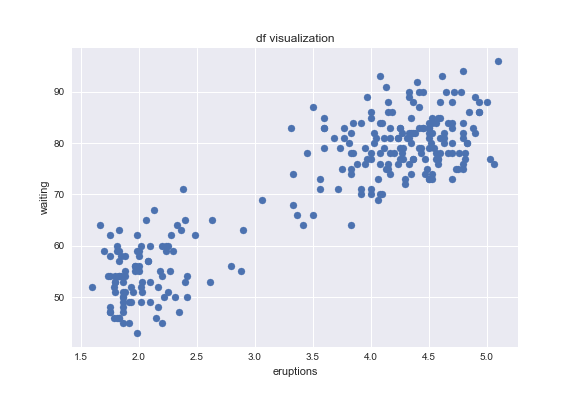
\includegraphics[width=0.8\textwidth]{df_visualization.png}
			\caption{visualization of \emph{faithful.csv} data}
		\end{figure}
	\item KMeans clustering visualization

		\begin{figure}
		     \centering
		     \begin{subfigure}[b]{0.6\textwidth}
		         \centering
		         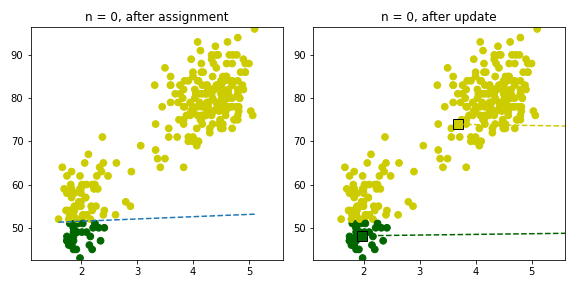
\includegraphics[width=\textwidth]{kmeans_visualization_0.png}
		         \caption{iteration = 0}
		     \end{subfigure}
		     \hfill
		     \begin{subfigure}[b]{0.6\textwidth}
		         \centering
		         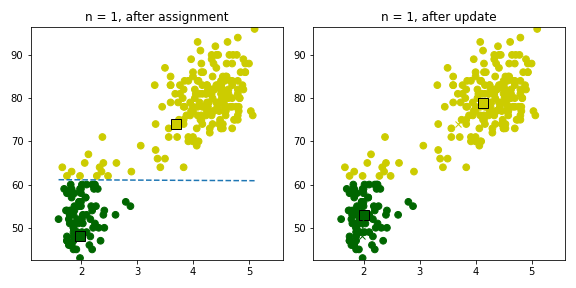
\includegraphics[width=\textwidth]{kmeans_visualization_1.png}
		         \caption{iteration = 1}
		     \end{subfigure}
		     \hfill
		     \begin{subfigure}[b]{0.6\textwidth}
		         \centering
		         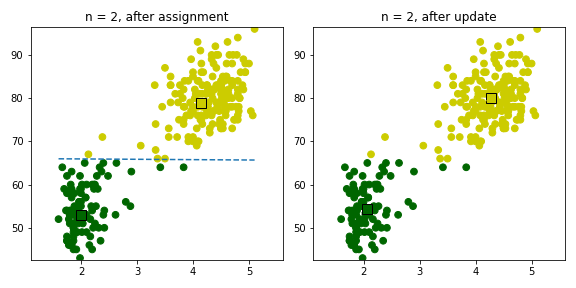
\includegraphics[width=\textwidth]{kmeans_visualization_2.png}
		         \caption{iteration = 2}
		     \end{subfigure}
		     \hfill
		     \begin{subfigure}[b]{0.6\textwidth}
		         \centering
		         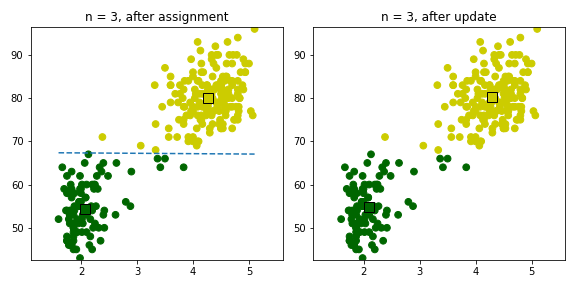
\includegraphics[width=\textwidth]{kmeans_visualization_3.png}
		         \caption{iteration = 3}
		     \end{subfigure}
		        \caption{KMeans algorithm}
		\end{figure}

		\begin{figure}
			\centering
			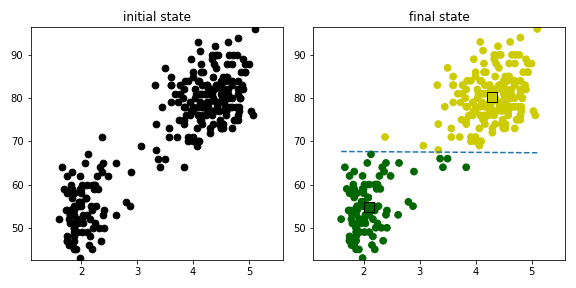
\includegraphics[width=0.8\textwidth]{kmeans_overall.png}
			\caption{KMean clustering sumup}
		\end{figure}
\end{enumerate}
\newpage
\exercise*[{[Implementing EM for Clustering]}]

\exercise*[{[Experiments with K-Means and EM]}]

\exercise*[{[Theory of K-means]}]

\begin{itemize}
	\item Show that the iterates of the algorithm satisfy
		\[\frac{1}{2}\sum_{k=1}^K \sum_{x\in C_k^{(i)}}\norm{x - m_k^{(i)}}^2 \leq
		\frac{1}{2}\sum_{k=1}^K \sum_{x\in C_k^{(i-1)}}\norm{x - m_k^{(i-1)}}^2 \]
		To confirm the inequality above we will show that both of operations can never increase the clustering energy.
		\[E(C^{(i)},m^{(i)}) \coloneqq \frac{1}{2}\sum_{k=1}^K \sum_{x\in C_k^{(i)}}\norm{x - m_k^{(i)}}^2 \triangleq \text{clustering energy}\]
		\begin{enumerate}
		\item $E(C^{(i)},m^{(i)}) < E(C^{(i-1)},m^{(i)})$
		
			From the logic of the algorithm: $C^{(i)}$ and $C^{(i-1)}$ are differently only if there is a point that finds a closer cluster center in $m^{(i)}$ than the one assigned to it by $C^{(i-1)}$.Hence, 
			\[\frac{1}{2}\sum_{k=1}^K \sum_{x\in C_k^{(i)}}\norm{x - m_k^{(i)}}^2 <
			\frac{1}{2}\sum_{k=1}^K \sum_{x\in C_k^{(i-1)}}\norm{x - m_k^{(i)}}^2 \]
		\item $E(C^{(i)},m^{(i)}) \leq E(C^{(i)},m^{(i-1)})$
			
			This statement is equivalent to the following
			\[\frac{1}{2}\sum_{k=1}^K \sum_{x\in C_k}\norm{x - m_k}^2 \leq
			\frac{1}{2}\sum_{k=1}^K \sum_{x\in C_k}\norm{x - a_k}^2 \]
			, where $a = (a_1, \dots, a_k)$ with $a_k \in \R^M$ is an arbitrary point in the same space. Consider $C_k$ for it:
			\[\sum_{x\in C_k}\norm{x - m_k}^2 \leq \sum_{x\in C_k}\norm{x - a_k}^2\]
			\begin{align*}
				\sum_{x\in C_k}\norm{x - a_k}^2 &= \sum_{x\in C_k}\norm{(x - m_k) + (x - a_k)}^2 \\
				& = \sum_{x\in C_k}\norm{x - m_k}^2 + \norm{m_k - a_k}^2 + 2(x - m_k)\cdot (m_k - a_k) \\
				& = \sum_{x\in C_k}\norm{x - m_k}^2 + \sum_{x\in C_k}\norm{m_k - a_k}^2 + 2\sum_{x\in C_k}(x\cdot m_k - x\cdot a_k - m_k \cdot m_k + m_k \cdot a_k) \\
				& \text{as} \sum_{x\in C_k} x = \sum_{x\in C_k} m_k \\
				& = \sum_{x\in C_k}\norm{x - m_k}^2 + |C_k|\norm{m_k - a_k}^2 + 2\cdot |C_k|(m_k \cdot m_k - m_k \cdot a_k - m_k\cdot m_k + m_k \cdot a_k) \\
				&= \sum_{x\in C_k}\norm{x - m_k}^2 + |C_k|\norm{m_k - a_k}^2 \\
				&\geq \sum_{x\in C_k}\norm{x - m_k}^2
			\end{align*}
		\end{enumerate}
		Hence,
		\[\frac{1}{2}\sum_{k=1}^K \sum_{x\in C_k^{(i)}}\norm{x - m_k^{(i)}}^2 \leq
		\frac{1}{2}\sum_{k=1}^K \sum_{x\in C_k^{(i-1)}}\norm{x - m_k^{(i-1)}}^2 \]
	\item Every data point $x_n$ must be assigned to precisely one class in oder to the algorithm be converging. It was shown above. 
	\item It is not a big deal to extend first step to an arbitrary norm. The problem is how to calculate centers of clusters.
	\item In that case result of clustering depends on realization in programm. Final result significantly depends on the initial statements of centers.
	\newpage
	\begin{figure}
		\centering
		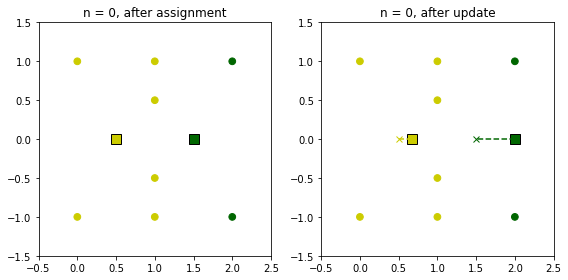
\includegraphics[width=0.8\textwidth]{kmeans_exercise_3_it.png}
		\caption{KMeans algorithm}
	\end{figure}
	\hfill
	\begin{figure}
		\centering
		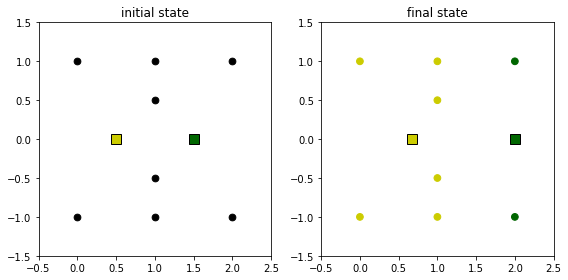
\includegraphics[width=0.8\textwidth]{kmeans_exercise_3_sumup.png}
		\caption{KMean clustering sumup}
	\end{figure}
\end{itemize}

\end{document}